\documentclass{article}
\usepackage[utf8]{inputenc}
\usepackage[T1]{fontenc}
\usepackage[export]{adjustbox}
\usepackage{mathtools,amsthm,amssymb,icomma,upgreek,xfrac,enumerate, bbm,titlesec,lmodern,polski,derivative,geometry,multicol,titling,graphicx,url,amsmath,caption,lipsum,float,longtable,booktabs}
\usepackage[table,xcdraw]{xcolor}
\usepackage[hidelinks,breaklinks,pdfusetitle,pdfdisplaydoctitle]{hyperref}
\usepackage{listings}
\definecolor{codegreen}{rgb}{0,0.6,0}
\definecolor{codegray}{rgb}{0.5,0.5,0.5}
\definecolor{codepurple}{rgb}{0.58,0,0.82}
\definecolor{backcolour}{rgb}{0.95,0.95,0.92}
\definecolor{light-gray}{gray}{0.95}
\setlength{\droptitle}{-1cm}
\mathtoolsset{showonlyrefs,mathic}
\title{Analiza danych rzeczywistych przy pomocy modelu ARMA}
\author{Natalia Klepacka, Joanna Kołaczek}
\date{\today}
\newtheoremstyle{break}
{\topsep}{\topsep}%
{\normalfont}{}%
{\bfseries}{}%
{\newline}{}%
\theoremstyle{break}

\titleformat*{\section}{\LARGE\bfseries}
\titleformat*{\subsection}{\Large\bfseries}
\titleformat*{\subsubsection}{\large\bfseries}
\titleformat*{\paragraph}{\large\bfseries}
\titleformat*{\subparagraph}{\large\bfseries}

\lstdefinestyle{mystyle}{
	backgroundcolor=\color{backcolour},   
	commentstyle=\color{codegreen},
	keywordstyle=\color{magenta},
	numberstyle=\tiny\color{codegray},
	stringstyle=\color{codepurple},
	basicstyle=\ttfamily\footnotesize,
	breakatwhitespace=false,         
	breaklines=true,                 
	captionpos=b,                    
	keepspaces=true,                 
	numbers=left,                    
	numbersep=5pt,                  
	showspaces=false,                
	showstringspaces=false,
	showtabs=false,                  
	tabsize=2
}

\lstset{style=mystyle}
\renewcommand{\lstlistingname}{Kod}% Listing -> Kod
\renewcommand{\lstlistlistingname}{Lista Kodów}% List of Listings -> Lista kodów
\newcommand{\code}[1]{\colorbox{light-gray}{\texttt{#1}}}

\graphicspath{{obrazki/}}


\begin{document}
	\maketitle
	\tableofcontents
	\clearpage
	\section{Wstęp}
	Niniejszy raport powstał na potrzeby realizacji laboratorium z Komputerowej Analizy Szeregów Czasowych, prowadzonych przez mgr Justynę Witulską, do wykładu prof. Agnieszki Wyłomańskiej.
	Będziemy analizować dane dotyczące średniej dziennej temperatury w Londynie, na przestrzeni lat 1979-1987. Dane pochodzą \href{https://www.kaggle.com/datasets/emmanuelfwerr/london-weather-data }{\textit{z tej strony}}. Są to informacje kolekcjonowane przez European Climate Assessment and Dataset - projekt zbierający dane o pogodzie w Europie.
	W raporcie przeprowadzimy dekompozycji Walda oraz przy pomocy kryteriów informacyjnych dobierzemy rzędy modelu ARMA, aby następnie wyestymować wartości parametrów tegoż modelu. Na koniec zweryfikujemy również, czy założenia dotyczące szumu są spełnione.
	
	Życzymy Czytelnikowi miłej lektury.
	
	\section{Przygotowanie danych do analizy}
	W rozważanym przez nas fragmencie danych, nie było żadnych braków danych ani wartości odstających, zatem analizujemy je w niezmienionej formie. Na wykresie [\ref{fig:p1}] przedstawiona jest zależność średniej dziennej temperatury w Londynie od czasu. Wyraźnie widoczna jest sezonowość, natomiast nie możemy być pewni co do obecności trendu. Wykresy autokorelacji [\ref{fig:acf1}] oraz częściowej autokorelacji [\ref{fig:pacf1}] potwierdzają, że nie możemy mówić tu o szeregu stacjonarnym.
	
	\begin{figure}[H]
		\begin{center}
			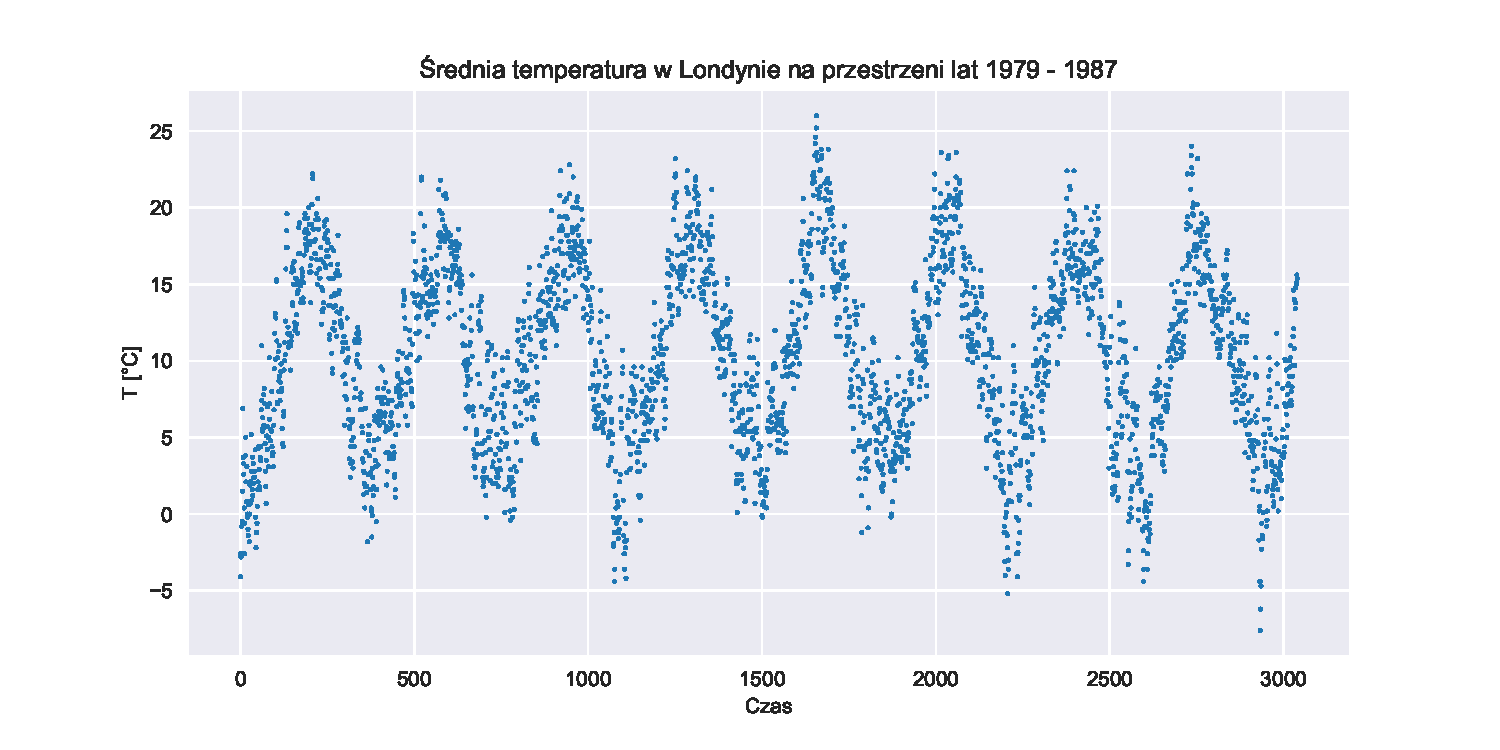
\includegraphics[scale=0.63]{plot1.pdf}
			\caption{Wykres temperatury w Londynie}
			\label{fig:p1}
		\end{center}
	\end{figure}
	
	\begin{figure}[H]
		\begin{center}
			\begin{minipage}{0.49\linewidth}
				\centering
				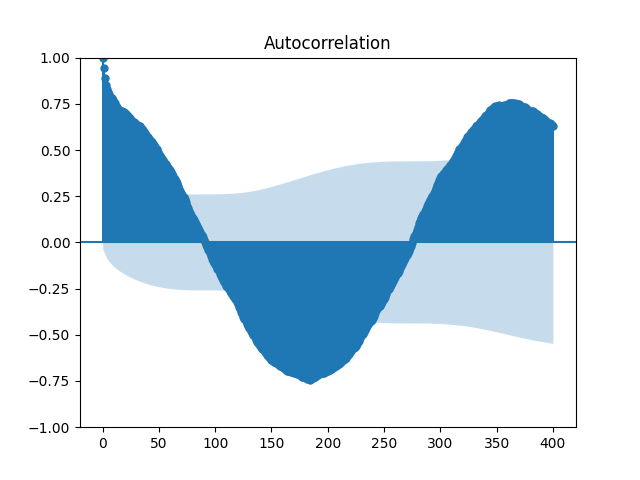
\includegraphics[scale=0.49]{acf1.png}
				\caption{Autokorelacja}
				\label{fig:acf1}
			\end{minipage}
			\begin{minipage}{0.49\linewidth}
				\centering
				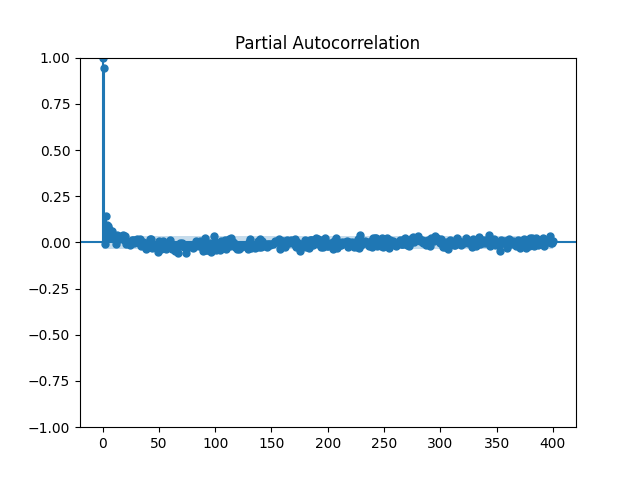
\includegraphics[scale=0.49]{pacf1.png}
				\caption{Częściowa autokorelacja}
				\label{fig:pacf1}
			\end{minipage}
		\end{center}
	\end{figure}
	
	Aby usunąć możliwy trend, stosujemy dla naszych danych regresję liniową. Efekt widzimy na wykresie [\ref*{fig:p2}]. Obliczony współczynnik kierunkowy był bardzo bliski 0, co oznacza, że w danych nie występuje trend liniowy. Wyraz wolny wyniósł około 10, więc odejmujemy tę wartość od wartości oryginalnych, aby ich średnia była bliska 0.
	
	\begin{figure}[H]
		\begin{center}
			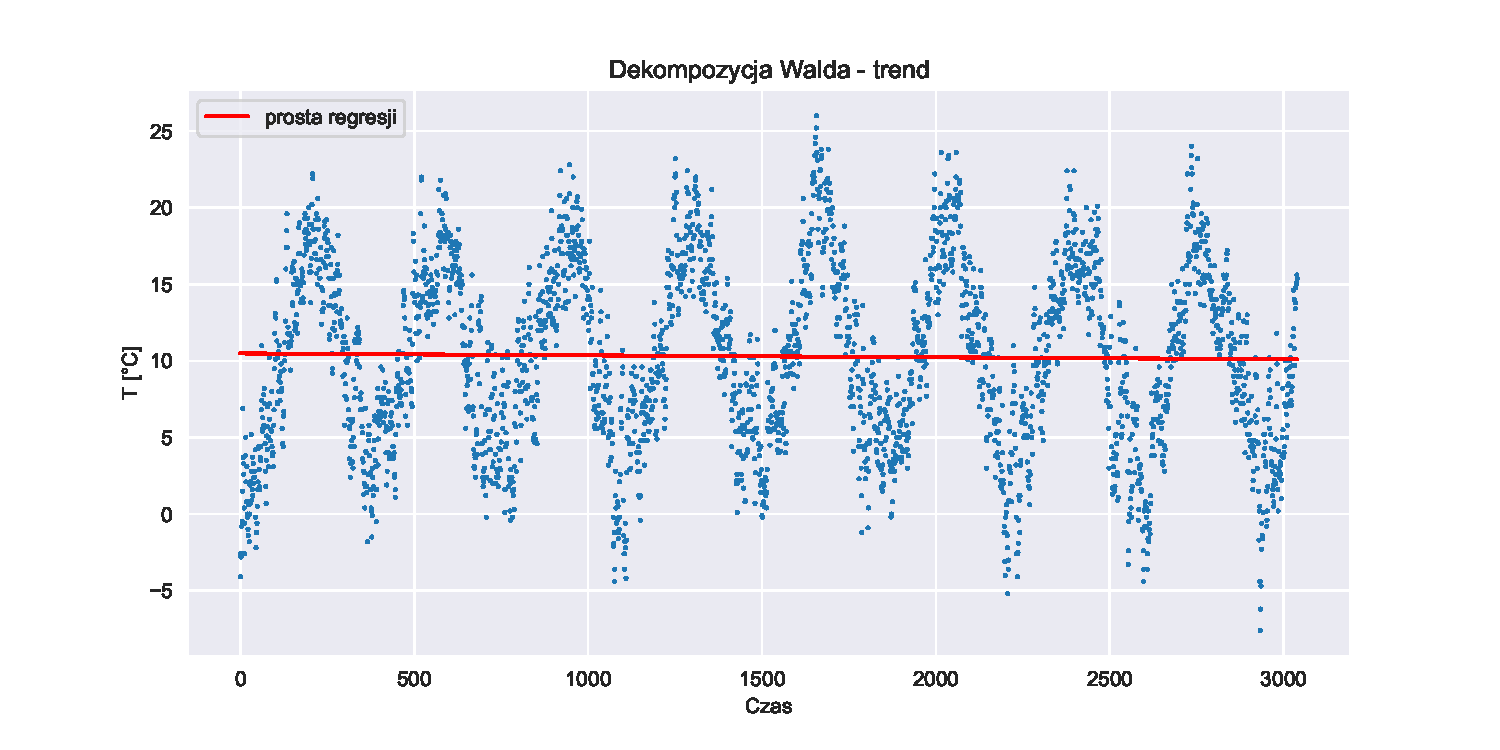
\includegraphics[scale=0.63]{plot2.pdf}
			\caption{Regresja liniowa}
			\label{fig:p2}
		\end{center}
	\end{figure}

\newpage
	
	Kolejnym krokiem będzie próba usunięcia sezonowości. Na poprzednich wykresach mogliśmy zauważyć, że dane układają się w kształt funkcji sinusoidalnej. Załóżmy, że da się je opisać przy pomocy funkcji $f(x) = c\cdot\sin(d\cdot x+e)$. Używamy pakietu \code{scipy}, a konkretnie funkcji \code{optimize.curve\_fit}, aby dopasować odpowiednie współczynniki $c$, $d$, $e$. Efekt widzimy na wykresie \ref{fig:p3}.
	
	\begin{figure}[H]
		\begin{center}
			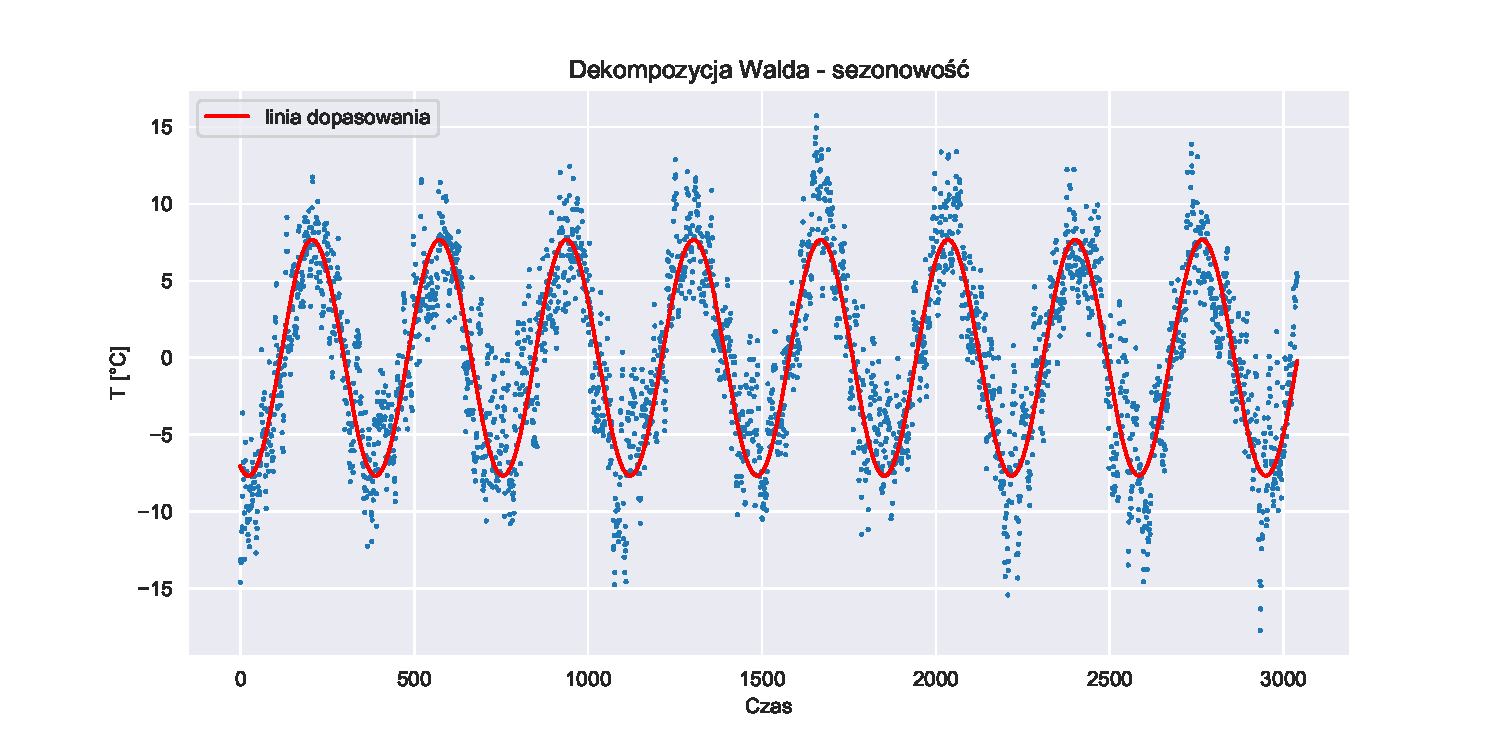
\includegraphics[scale=0.5]{plot3.pdf}
			\caption{Krzywa sinusoidalna}
			\label{fig:p3}
		\end{center}
	\end{figure}
	
	Aby dokończyć proces dekompozycji, wystarczy od naszych danych odjąć wartości otrzymanej funkcji w danym czasie [\ref{fig:p4}]. Możemy teraz ponownie sprawdzić, jak prezentują się wykresy autokorelacji i częściowej autokorelacji. Od tego momentu będziemy zakładać, że szereg czasowy jest stacjonarny w słabym sensie.
	
	\begin{figure}[H]
		\begin{center}
			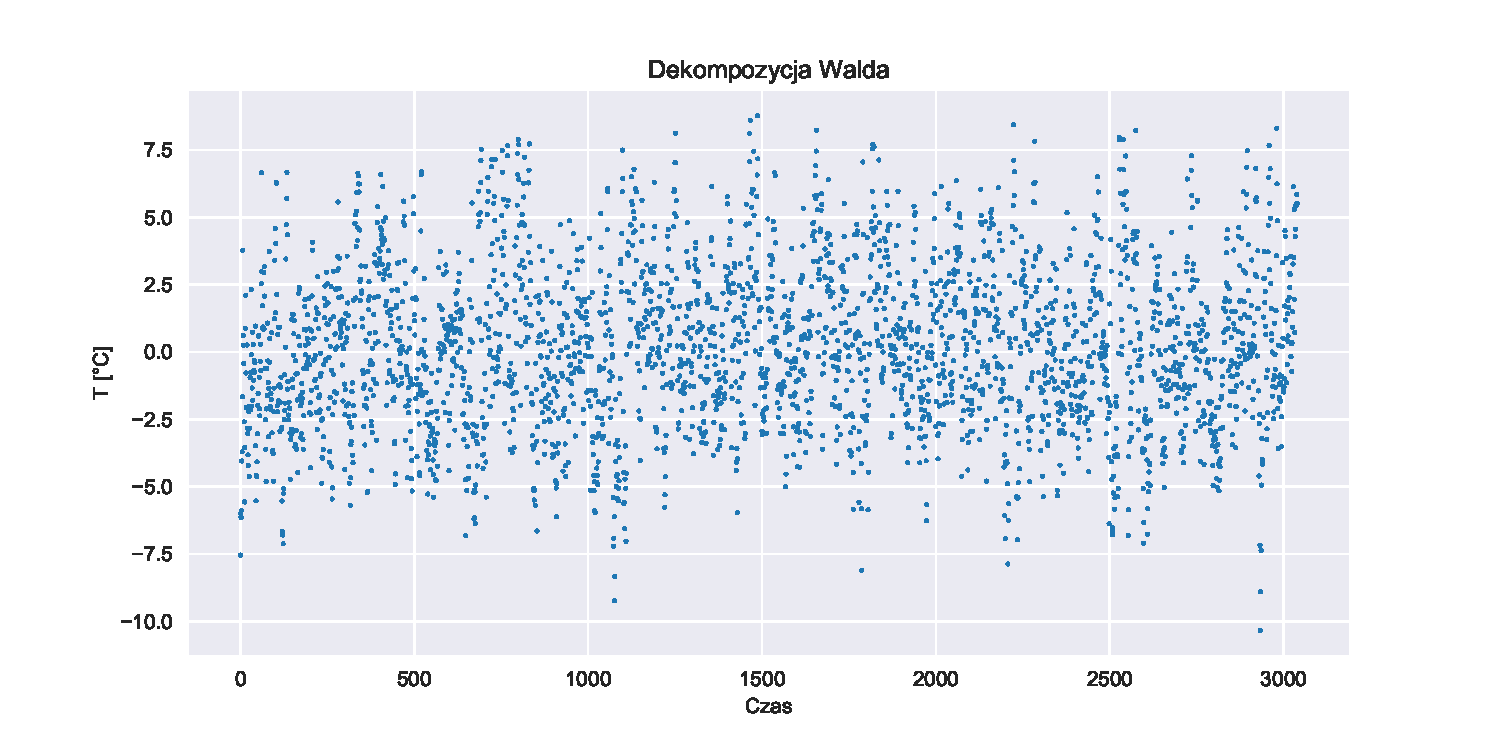
\includegraphics[scale=0.5]{plot4.pdf}
			\caption{Dane po dekompozycji}
			\label{fig:p4}
		\end{center}
	\end{figure}
	
	\begin{figure}[H]
		\begin{center}
			\begin{minipage}{0.49\linewidth}
				\centering
				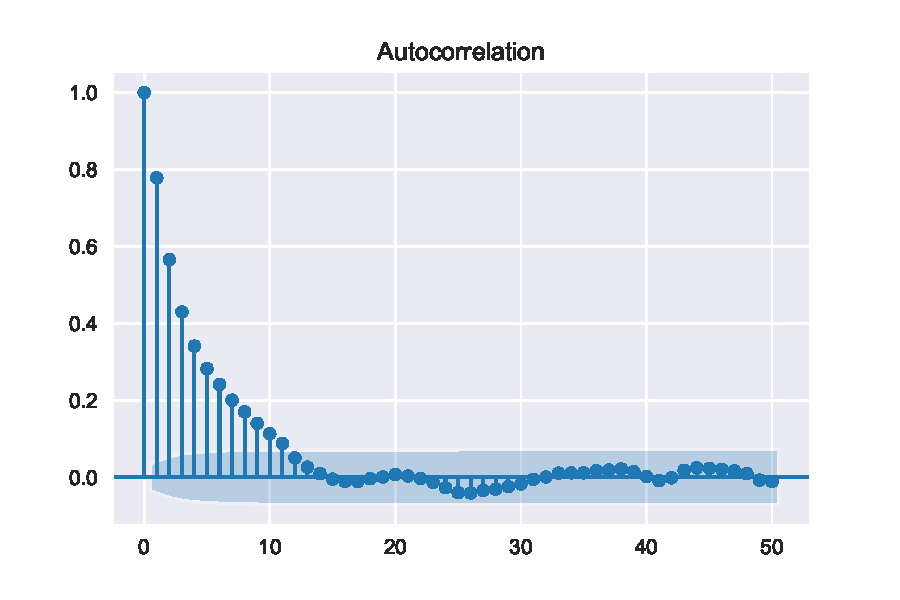
\includegraphics[scale=0.49]{acf2.pdf}
				\caption{Autokorelacja}
				\label{fig:acf2}
			\end{minipage}
			\begin{minipage}{0.49\linewidth}
				\centering
				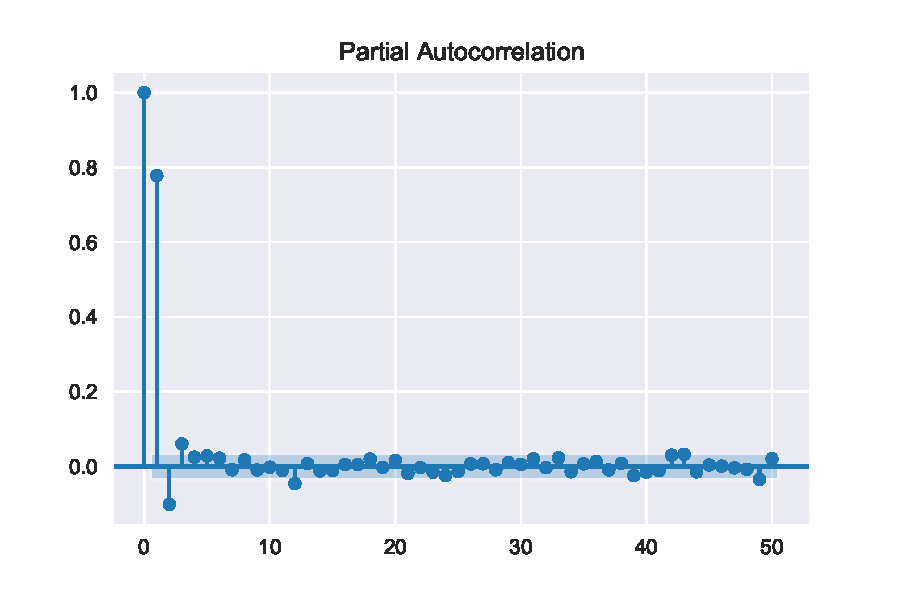
\includegraphics[scale=0.49]{pacf2.pdf}
				\caption{Częściowa autokorelacja}
				\label{fig:pacf2}
			\end{minipage}
		\end{center}
	\end{figure}
	
	\section{Modelowanie danych przy pomocy ARMA}
	
	\subsection{Dobór rzędu modelu}
	W celu dobrania rzędu modelu wyliczyłyśmy wartości kryteriów informacyjnych
	\begin{itemize}
		\item Kryterium Informacyjne Akaikego (AIC),
		\item Bayesowskie Kryterium Informacyjne (BIC),
		\item Kryterium Informacyjne Hannana-Quinna (HQIC)
	\end{itemize}
	
	dla wartości $p$ i $q$ z przedziału $[0,9]$. Otrzymałyśmy winiki widoczne w tabelach [\ref{t1}][\ref{t2}][\ref{t3}]. Najlepiej dopasowane pary wg poszczególnych kryteriów to
	
	\begin{itemize}
		\item $p=5$, $q=6$ dla AIC,
		\item $p=1$, $q=1$ dla BIC,
		\item $p=3$, $q=0$ dla HQIC.
	\end{itemize}
	
	Jako że nie da się określić modelu jednoznacznie najlepiej dopasowanego, do dalszej analizy zdecydowałyśmy się przyjąć najmniej skomplikowany model, czyli ARMA(1, 1).
	
	\begin{table}[H]
		\centering
		\begin{tabular}{|r|r|r|r|r|}
			\hline
			\rowcolor[HTML]{C0C0C0} 
			{\color[HTML]{343434} \textbf{p}} & {\color[HTML]{343434} \textbf{q}} & {\color[HTML]{343434} \textbf{AIC}} & {\color[HTML]{343434} \textbf{BIC}} & {\color[HTML]{343434} \textbf{HQIC}} \\ \hline
			{\color[HTML]{343434} 5}          & {\color[HTML]{343434} 6}          & {\color[HTML]{343434} 10933.960861} & {\color[HTML]{343434} 11010.577298} & {\color[HTML]{343434} 10961.678129}  \\ \hline
			{\color[HTML]{343434} 7}          & {\color[HTML]{343434} 8}          & {\color[HTML]{343434} 10934.090625} & {\color[HTML]{343434} 11034.281350} & {\color[HTML]{343434} 10970.336283}  \\ \hline
			{\color[HTML]{343434} 9}          & {\color[HTML]{343434} 7}          & {\color[HTML]{343434} 10934.984168} & {\color[HTML]{343434} 11041.068465} & {\color[HTML]{343434} 10973.361923}  \\ \hline
			{\color[HTML]{343434} 7}          & {\color[HTML]{343434} 9}          & {\color[HTML]{343434} 10935.015702} & {\color[HTML]{343434} 11041.100000} & {\color[HTML]{343434} 10973.393458}  \\ \hline
			{\color[HTML]{343434} 4}          & {\color[HTML]{343434} 4}          & {\color[HTML]{343434} 10935.166047} & {\color[HTML]{343434} 10994.101768} & {\color[HTML]{343434} 10956.487023}  \\ \hline
		\end{tabular}
		\caption{Kryteria informacyjne wg AIC}
		\label{t1}
	\end{table}
	
	\begin{table}[H]
		\centering
		\begin{tabular}{|r|r|r|r|r|}
			\hline
			\rowcolor[HTML]{C0C0C0} 
			{\color[HTML]{111111} \textbf{p}} & {\color[HTML]{111111} \textbf{q}} & {\color[HTML]{111111} \textbf{AIC}} & {\color[HTML]{111111} \textbf{BIC}} & {\color[HTML]{111111} \textbf{HQIC}} \\ \hline
			\rowcolor[HTML]{FFFFFF} 
			{\color[HTML]{111111} 1}          & {\color[HTML]{111111} 1}          & {\color[HTML]{111111} 10945.997929} & {\color[HTML]{111111} 10969.572218} & {\color[HTML]{111111} 10954.526320}  \\ \hline
			\rowcolor[HTML]{FFFFFF} 
			{\color[HTML]{111111} 3}          & {\color[HTML]{111111} 0}          & {\color[HTML]{111111} 10940.398608} & {\color[HTML]{111111} 10969.866469} & {\color[HTML]{111111} 10951.059096}  \\ \hline
			\rowcolor[HTML]{FFFFFF} 
			{\color[HTML]{111111} 1}          & {\color[HTML]{111111} 2}          & {\color[HTML]{111111} 10941.710972} & {\color[HTML]{111111} 10971.178832} & {\color[HTML]{111111} 10952.371459}  \\ \hline
			\rowcolor[HTML]{FFFFFF} 
			{\color[HTML]{111111} 2}          & {\color[HTML]{111111} 1}          & {\color[HTML]{111111} 10944.132071} & {\color[HTML]{111111} 10973.599931} & {\color[HTML]{111111} 10954.792559}  \\ \hline
			\rowcolor[HTML]{FFFFFF} 
			{\color[HTML]{111111} 2}          & {\color[HTML]{111111} 2}          & {\color[HTML]{111111} 10938.737268} & {\color[HTML]{111111} 10974.098700} & {\color[HTML]{111111} 10951.529853}  \\ \hline
		\end{tabular}
		\caption{Kryteria informacyjne wg BIC}
		\label{t2}
	\end{table}
	
	\begin{table}[H]
		\centering
		\begin{tabular}{|r|r|r|r|r|}
			\hline
			\rowcolor[HTML]{C0C0C0} 
			{\color[HTML]{111111} \textbf{p}} & {\color[HTML]{111111} \textbf{q}} & {\color[HTML]{111111} \textbf{AIC}} & {\color[HTML]{111111} \textbf{BIC}} & {\color[HTML]{111111} \textbf{HQIC}} \\ \hline
			{\color[HTML]{111111} 3}          & {\color[HTML]{111111} 0}          & {\color[HTML]{111111} 10940.398608} & {\color[HTML]{111111} 10969.866469} & {\color[HTML]{111111} 10951.059096}  \\ \hline
			{\color[HTML]{111111} 2}          & {\color[HTML]{111111} 2}          & {\color[HTML]{111111} 10938.737268} & {\color[HTML]{111111} 10974.098700} & {\color[HTML]{111111} 10951.529853}  \\ \hline
			{\color[HTML]{111111} 3}          & {\color[HTML]{111111} 1}          & {\color[HTML]{111111} 10938.935705} & {\color[HTML]{111111} 10974.297137} & {\color[HTML]{111111} 10951.728290}  \\ \hline
			{\color[HTML]{111111} 1}          & {\color[HTML]{111111} 2}          & {\color[HTML]{111111} 10941.710972} & {\color[HTML]{111111} 10971.178832} & {\color[HTML]{111111} 10952.371459}  \\ \hline
			{\color[HTML]{111111} 1}          & {\color[HTML]{111111} 3}          & {\color[HTML]{111111} 10940.538468} & {\color[HTML]{111111} 10975.899900} & {\color[HTML]{111111} 10953.331053}  \\ \hline
		\end{tabular}
		\caption{Kryteria informacyjne wg HQIC}
		\label{t3}
	\end{table}
	
	Jako że nie da się określić modelu jednoznacznie najlepiej dopasowanego, do dalszej analizy zdecydowałyśmy się przyjąć najmniej skomplikowany model, czyli ARMA(1, 1).
	
	\subsection{Estymacja parametrów modelu}
	Do estymacji parametrów wykorzystamy metodę największej wiarygodności zaimplementowaną w pythonowym pakiecie \code{statsmodels}. Metoda ta zakłada, że zmienne składające się na szum mają rozkład normalny. Wartości współczynników można zobaczyć w tabeli [\ref{t4}]
	
	\begin{table}[H]
		\centering
		\begin{tabular}{l|l|l|l|l|l|l|}
			\cline{2-7}
			& \cellcolor[HTML]{C0C0C0}coef & \cellcolor[HTML]{C0C0C0}std err & \cellcolor[HTML]{C0C0C0}z & \cellcolor[HTML]{C0C0C0}P\textgreater{}|z| & \cellcolor[HTML]{C0C0C0}{[}0.025 & \cellcolor[HTML]{C0C0C0}0.975{]} \\ \hline
			\multicolumn{1}{|l|}{\cellcolor[HTML]{C0C0C0}{\color[HTML]{111111} const}}  & 0.2230                       & 0.150                           & 1.486                     & 0.137                                      & -0.071                           & 0.517                            \\ \hline
			\multicolumn{1}{|l|}{\cellcolor[HTML]{C0C0C0}{\color[HTML]{111111} ar.L1}}  & 0.7205                       & 0.017                           & 42.821                    & 0.000                                      & 0.687                            & 0.753                            \\ \hline
			\multicolumn{1}{|l|}{\cellcolor[HTML]{C0C0C0}{\color[HTML]{111111} ma.L1}}  & 0.1546                       & 0.023                           & 6.580                     & 0.000                                      & 0.109                            & 0.201                            \\ \hline
			\multicolumn{1}{|l|}{\cellcolor[HTML]{C0C0C0}{\color[HTML]{111111} sigma2}} & 3.4663                       & 0.096                           & 35.996                    & 0.000                                      & 3.278                            & 3.655                            \\ \hline
		\end{tabular}
		\caption{Współczynniki modelu}
		\label{t4}
	\end{table}
	
	\section{Ocena dopasowania modelu}
	\begin{figure}[H]
		\begin{center}
			\begin{minipage}{0.49\linewidth}
				\centering
				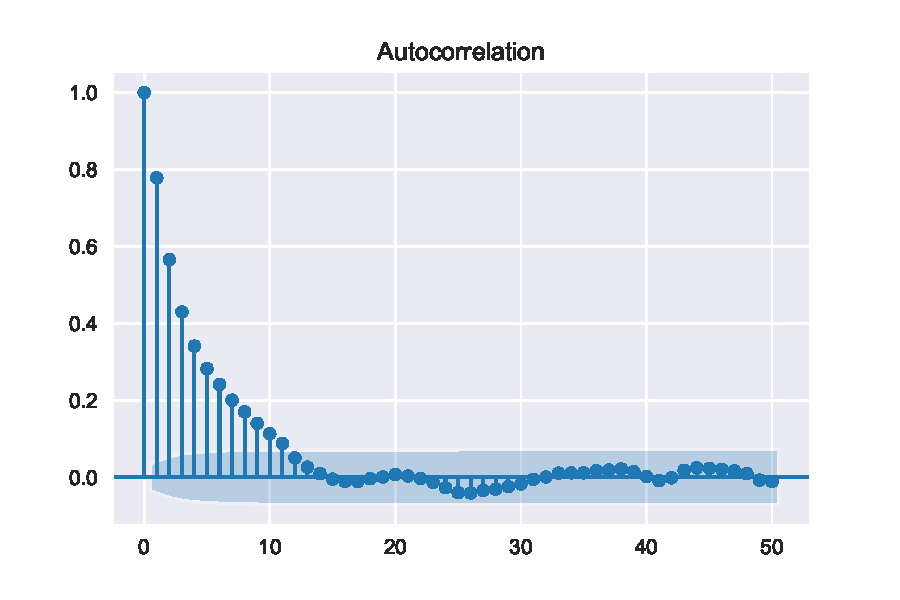
\includegraphics[scale=0.49]{acf2.pdf}
				\caption{Autokorelacja}
				\label{fig:acf2}
			\end{minipage}
			\begin{minipage}{0.49\linewidth}
				\centering
				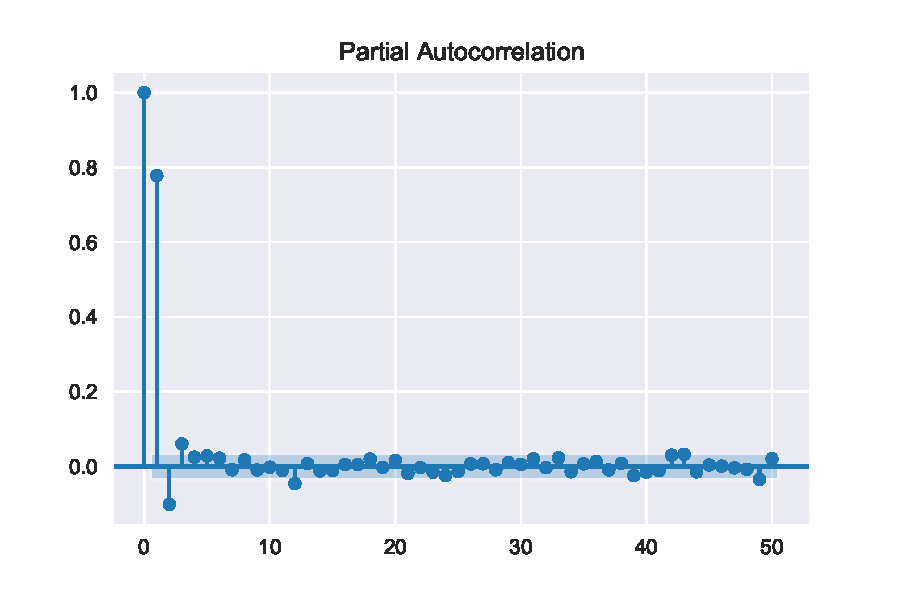
\includegraphics[scale=0.49]{pacf2.pdf}
				\caption{Częściowa autokorelacja}
				\label{fig:pacf2}
			\end{minipage}
		\end{center}
	\end{figure}
	
	Od pewnego momentu wszystkie wartości funkcji autokorelacji i częściowej autokorelacji mieszczą się w przedziałach ufności, co sugeruje, że model jest dobrze dopasowany do danych.
	
	
	\section{Weryfikacja założeń dotyczących szumu}
	
	Szum ${Z_t}$ w modelu ARMA powinien spełniać poniższe założenia:
	\begin{enumerate}
		\item Średnia ${Z_t}$ jest bliska 0
		\item Wariancja ${Z_t}$ jest taka sama dla każdego $t$
		\item ${Z_t}$ są niezależne
		\item ${Z_t}$ mają rozkład normalny
	\end{enumerate}
	
	\begin{figure}[H]
		\begin{center}
			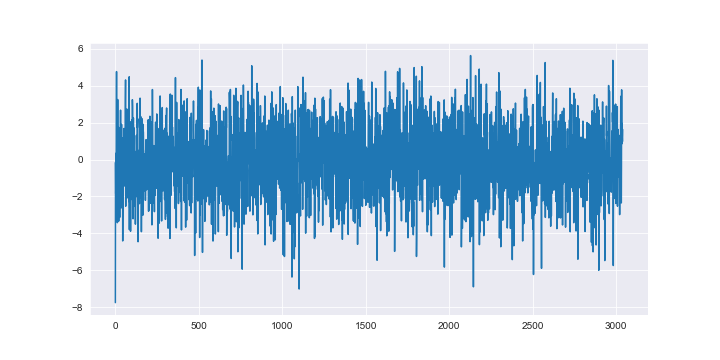
\includegraphics[scale=0.63]{res.png}
			\caption{Residua modelu}
			\label{fig:res}
		\end{center}
	\end{figure}
	
	\subsection{Średnia}
	Na podstawie wykresu [\ref{fig:res}] możemy stwierdzić, że średnia prawdopodobnie jest równa 0. Dodatkowym sprawdzeniem może być wykonanie testu t. Test ten sprawdza hipotezę zerową "Średnia z próby jest równa $\mu$" przeciwko hipotezie alternatywnej "Średnia z próby jest różna od $\mu$". Jak widać poniżej [\ref{srednia}], wynik testu potwierdza wnioski wyciągnięte z wykresu — nie ma podstaw do odrzucenia hipotezy zerowej.
	
	\begin{lstlisting}[language=Python, caption=Test t, label={srednia}]
		sp.stats.ttest_1samp(resid, popmean=0)
		
		#output
		Ttest_1sampResult(statistic=0.04706184306961072, pvalue=0.9624674462497231)\end{lstlisting}
	
	\subsection{Wariancja}
	Na wykresie [\ref{fig:res}] nie widać znaczących zmian w wariancji zależnych od czasu, jednak dla pewności wykonamy test Levene'a jednorodności wariancji. Test ten sprawdza hipotezę zerową "Wszystkie próbki pochodzą z populacji o tej samej wariancji" przeciwko hipotezie alternatywnej "Przynajmniej dwie próbki pochodzą z populacji o różnych wariancjach". W tym celu dzieli próbkę na mniejsze podgrupy i porównuje ze sobą ich mediany.
	
	\begin{lstlisting}[language=Python, caption=Test Levene'a, label={var}]
		stat, p_value = scipy.stats.levene(random.sample(model.resid,500),random.sample(model.resid,500))
		if p_value > 0.05:
		print("Wariancja jest raczej stala.")
		else:
		print("Wariancja raczej nie jest stala.")
		
		#output
		Wariancja jest raczej stala.\end{lstlisting}
	
	Zgodnie z wynikiem testu [\ref{var}] nie ma podstaw do odrzucenia hipotezy zerowej, zatem możemy przyjąć, że wariancja residuów prawdopodobnie jest stała.
	
	\subsection{Niezależność}
	Z wykresów funkcji autokorelacji [\ref{fig:acf_res}] i częściowej autokorelacji [\ref{fig:pacf_res}] można łatwo wywnioskować, że residua są realizacjami niezależnych zmiennych losowych.
	
	\begin{figure}[H]
		\begin{center}
			\begin{minipage}{0.49\linewidth}
				\centering
				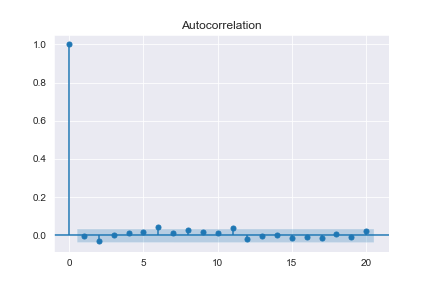
\includegraphics[scale=0.49]{acf_res.png}
				\caption{Autokorelacja}
				\label{fig:acf_res}
			\end{minipage}
			\begin{minipage}{0.49\linewidth}
				\centering
				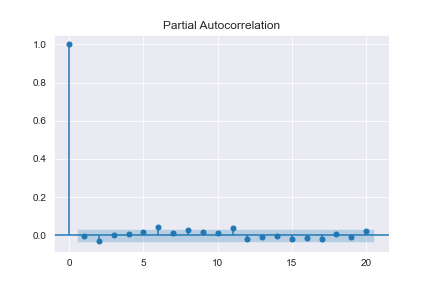
\includegraphics[scale=0.49]{pacf_res.png}
				\caption{Częściowa autokorelacja}
				\label{fig:pacf_res}
			\end{minipage}
		\end{center}
	\end{figure}
	
	Dystrybuanta rozkładu residuów niemal idealnie pokrywa się z dystrybuantą rozkładu normalnego [\ref{fig:res_dist}]. Podobnie histogram wartości [\ref{fig:res_pdf}] dobrze przybliża teoretyczną gęstość. Wykres kwantylowy [\ref{fig:res_qq}] pokrywa się odrobinę gorzej, ale nadal wystarczająco dobrze, żebyśmy mogli uznać, że dane pochodzą z rozkładu normalnego.
	
	\begin{figure}[H]
		\begin{center}
			\begin{minipage}{0.49\linewidth}
				\centering
				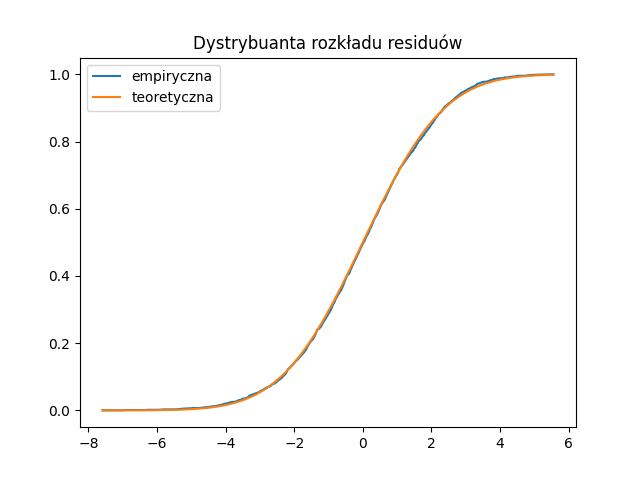
\includegraphics[scale=0.5]{res_dist.png}
				\caption{Dystrybuanta residuów}
				\label{fig:res_dist}
			\end{minipage}
			\begin{minipage}{0.49\linewidth}
				\centering
				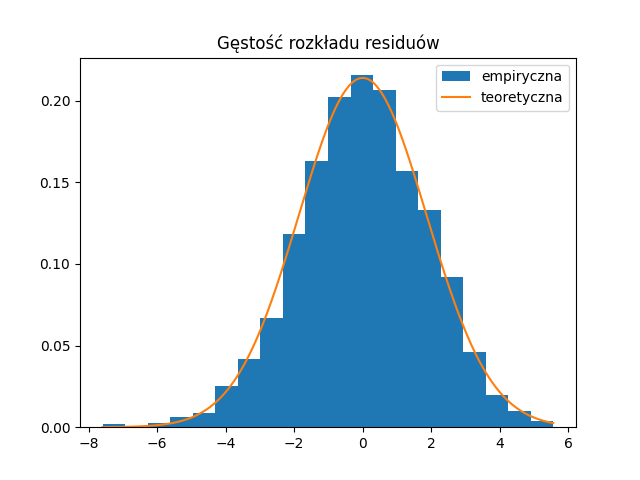
\includegraphics[scale=0.5]{res_pdf.png}
				\caption{Gęstość residuów}
				\label{fig:res_pdf}
			\end{minipage}
		\end{center}
	\end{figure}
	


	\begin{figure}[H]
		\begin{center}
			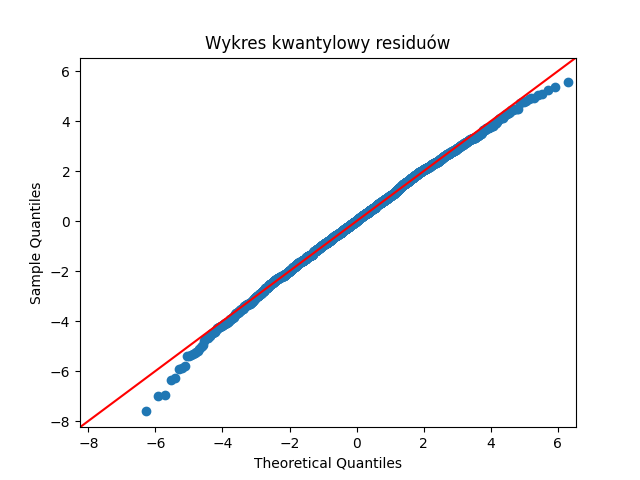
\includegraphics[scale=0.55]{res_qq.png}
			\caption{Wykres kwantylowy}
			\label{fig:res_qq}
		\end{center}
	\end{figure}
	
	\section{Podsumowanie}
	
	Na podstawie przeprowadzonej analizy możemy stwierdzić, że dane dotyczące średniej dziennej temperatury w Londynie, po przeprowadzeniu dekompozycji Walda, można opisać przy pomocy modelu ARMA. Dla modelu ARMA(1,1) residua spełniają wszystkie założenia co sugeruje, że jest on dobrze dopasowany. Otrzymane wyniki pozwalają predykować przyszłe wartości jednak należy pamiętać, że nasze przewidywania nigdy nie będą w stu procentach zgodne z rzeczywistością.
	
	\section{Źródła}
	\begin{itemize}
		\item Wykłady
		\item Dokumentacja pakietów \code{statsmodels} i \code{scipy}
		\item \url{}
		\item \url{https://www.kaggle.com/datasets/emmanuelfwerr/london-weather-data}
		\item \url{https://en.wikipedia.org/wiki/Student%27s_t-test}
		\item \url{https://en.wikipedia.org/wiki/Levene%27s_test}
		
	\end{itemize}
	
	
\end{document}